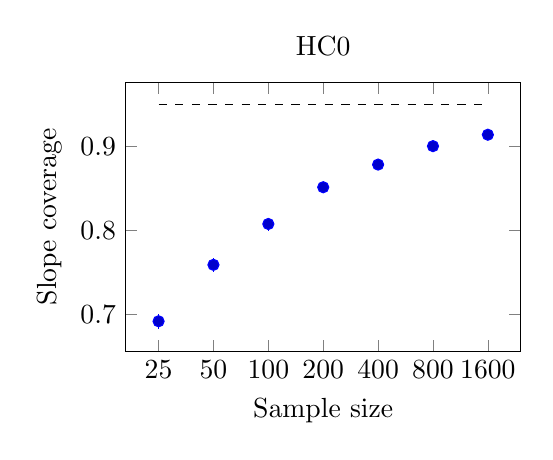
\begin{tikzpicture}
\begin{axis}[width=6.6cm,height=5cm,xlabel={Sample size},ylabel={Slope coverage},title={HC0},xtick={0,1,2,3,4,5,6},xticklabels={{25},{50},{100},{200},{400},{800},{1600}}]
% Interval meaning: Wilson 95% interval for coverage over 10000 trials
\addplot+[no marks,forget plot] coordinates {(0,0.6825768848970969) (0,0.7006758901275857)};
\addplot+[no marks,forget plot] coordinates {(1,0.7505189879210942) (1,0.7672821009228953)};
\addplot+[no marks,forget plot] coordinates {(2,0.7998580583286615) (2,0.815305629074024)};
\addplot+[no marks,forget plot] coordinates {(3,0.8443955232747883) (3,0.8583345258706262)};
\addplot+[no marks,forget plot] coordinates {(4,0.8719508884456331) (4,0.8847584247877647)};
\addplot+[no marks,forget plot] coordinates {(5,0.8944785166197612) (5,0.9062139006853268)};
\addplot+[no marks,forget plot] coordinates {(6,0.908447599852065) (6,0.9194343726973405)};
\addplot+[only marks,forget plot] coordinates {(0,0.6917) (1,0.759) (2,0.8077) (3,0.8515) (4,0.8785) (5,0.9005) (6,0.9141)};
\addplot[black,dashed,no marks,forget plot] coordinates {(0,0.95) (6,0.95)};
\end{axis}
\end{tikzpicture}
